\pagebreak
\section{Advection-Diffusion}
Apply the finite-difference method to solve the steady advection-diffusion equation with a source term,

\begin{equation*}
    u_x - \nu u_{xx} = \sin{\left(\pi x\right)}, \qquad u(0)=u(1)=0.
\end{equation*}

Write a code to solve this problem on a uniform grid of $N$ intervals.  Use central difference formulas for  both  the  first  and  second  derivatives. Using $N$=  16,  plot  the  solution  for $\nu$=  0.1  and $\nu$=  1 on one figure.  For $\nu$= 0.1, run simulations using $N= 4,\ 8,\ 16,\ 32$, and plot these on a single figure. Comment on the effect of $\nu$ and $N$ on the solution.  Also state whether and why the solution makes sense physically, based on your understanding of advection-diffusion.

\begin{adjustwidth}{2.5em}{0pt}        
\begin{align*}
    \shortintertext{Firstly, re-writing the equation above in finite terms gives,}
    u_x \approx \frac{u_{i+1} - u_{i-1}}{2\Delta x} & \\
    u_{xx}  \approx \frac{u_{i+1} - 2u_i + u_{i+1}}{\Delta x^2} & \\
    \shortintertext{Substituting into the given equation gives,}
    \underbrace{\frac{ u_{i+1} - u_{i-1}}{2\Delta x}}_{u_x} - \nu \underbrace{\frac{u_{i+1} - 2u_i + u_{i-1}}{\Delta x^2}}_{u_{xx}} & = \sin{(\pi x)}\\
    \shortintertext{Simplifying and grouping terms gives,}
    (\Delta x - 2\nu)u_{i+1} + 4\nu u_i - (\Delta x + 2\nu)u_{i-1} & = 2\Delta x^2\sin{(\pi x)}
    \shortintertext{Implementing these into Python and running the simulation gives,}
\end{align*}

\begin{figure}[h]
    \centering
    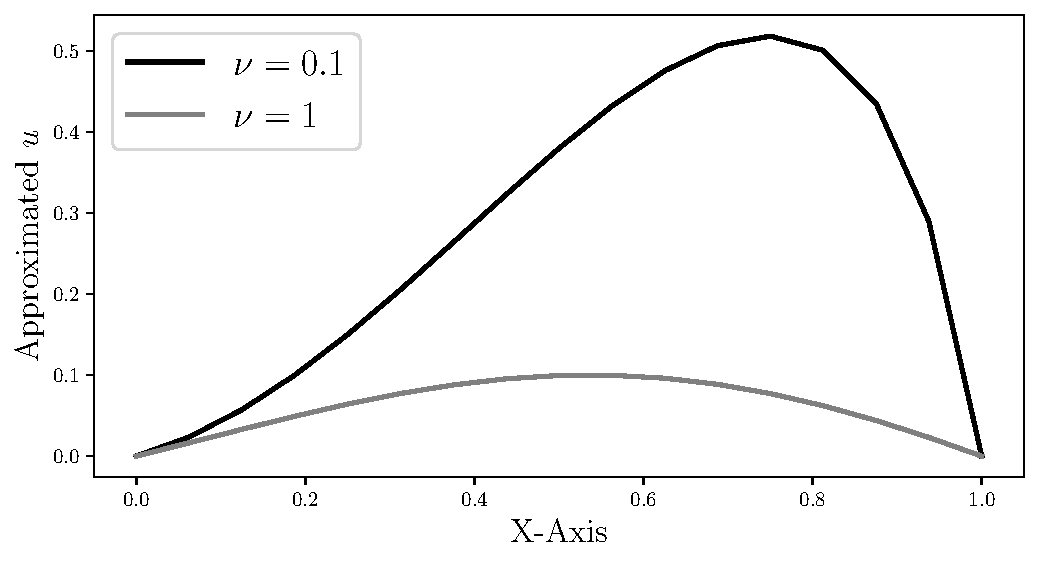
\includegraphics[width = 0.8\linewidth]{q5/nu_values.pdf}
    \caption{Advection-diffusion with varying $\nu$ values.}
    \label{fig:nu_vals}
\end{figure}
\end{adjustwidth}

\pagebreak

\begin{adjustwidth}{2.5em}{0pt}      
Doing so again but varying $N$

\begin{figure}[h]
    \centering
    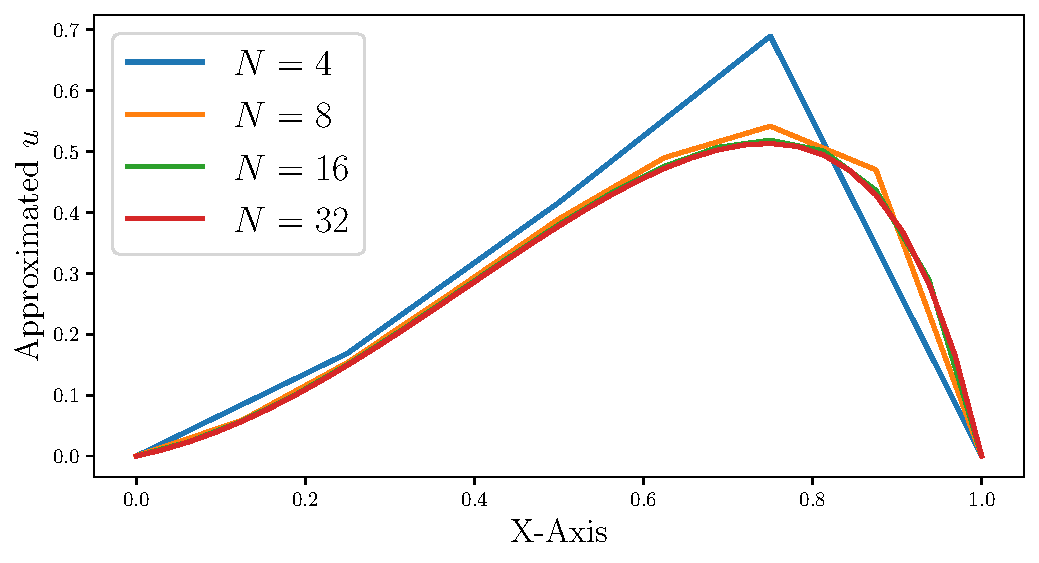
\includegraphics[width = 0.8\linewidth]{q5/varying_Ns.pdf}
    \caption{Advection-diffusion with varying $N$ values.}
    \label{fig:N_vals}
\end{figure}


\begin{fminipage}{0.8\linewidth}
    \textbf{Looking to Figures \ref{fig:nu_vals}, \ref{fig:N_vals} above we can observe the differences from varying $\bf N,$ and $\bf \nu$. Varying $\bf N$ only affects the \underline{refinment} of the simulation whereas varying $\bf \nu$ varies the \underline{physics} of the problem. With a higher $\bf \nu$ value, the more the approximated solution will match the point-source since the medium is more likely to diffuse to match the point source.}
\end{fminipage}
    
\end{adjustwidth}